\originalsection{曲线、坐标与局部微分}\label{tb:coordinates}
把位置写成球坐标, 有$x=r\sin\theta\cos\phi$, $y=r\sin\theta\sin\phi$, $z=r\cos\theta$. 因而$\rr=r\uv r$, 但位移微元还含角度变化:
\[
\dd\rr=\uv r\dd r+\uv\theta\,r\dd\theta
 +\uv\phi\,r\sin\theta\dd\phi.
\]
三个方向的单位矢量具体为
\begin{align*}
\uv r&=(\sin\theta\cos\phi,\sin\theta\sin\phi,\cos\theta),\\
\uv\theta&=(\cos\theta\cos\phi,\cos\theta\sin\phi,-\sin\theta),\\
\uv\phi&=(-\sin\phi,\cos\phi,0).
\end{align*}
它们依次指向径向增大、极角增大和方位角增大, 相互正交且长度为1.
这可以对三个直角分量分别求微分, 再按三个单位矢量分组得到. 所以沿极角方向走$\dd\theta$的实际弧长是$r\dd\theta$, 不能把$\dd\theta$直接当长度. 对$\dd V=\nabla V\cdot\dd\rr$, 比较每个微分的系数, 得
\[
\nabla V=\uv r\partial_rV+\uv\theta\frac1r\partial_\theta V
 +\uv\phi\frac1{r\sin\theta}\partial_\phi V.
\]
柱坐标同理给$\dd\rr=\uv s\dd s+\uv\phi s\dd\phi+\uv z\dd z$和$\nabla V=\uv s\partial_sV+\uv\phi\partial_\phi V/s+\uv z\partial_zV$. 这些尺度因子解释了后文偶极势求场时为何角向导数要除以$r$. 轴与极点的坐标奇点需另用连续直角分量判断, 不能把坐标分母为零等同于真实场奇点.

\begin{example}\label{ex:scalarplots}
原1.10.2比较$f_1=1/r$和$f_2=1/\sqrt{x^2+(y-1)^2}-1/\sqrt{x^2+(y+1)^2}$. 给出其零点、奇点、对称与图形意义.
\end{example}
\begin{solution}
$f_1$以原点为中心, 等值线为半径$1/f_1$的圆; 高度随$r$增加下降, 原点有正无穷奇点. $f_2$在$(0,1)$有正奇点, 在$(0,-1)$有负奇点, 对$x$为偶、对$y$为奇, 整条$y=0$为零. 它类似两个异号点源的势; 等势线并非源的运动轨迹. 函数只依赖所显示二维位置, 若把它解释成三维点电荷势的切面, 原三维表达式仍需补$z^2$. 奇点不能靠选几个采样点证明消失.
\end{solution}
\begin{center}
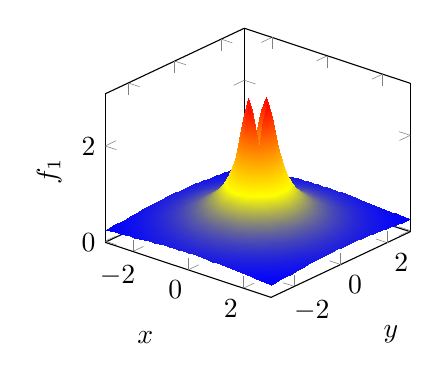
\begin{tikzpicture}
\begin{axis}[width=.45\linewidth,height=5cm,view={40}{30},xlabel={$x$},ylabel={$y$},zlabel={$f_1$},domain=-3:3,y domain=-3:3,samples=35,samples y=35,unbounded coords=jump]
\addplot3[surf,shader=interp] {x^2+y^2>.09 ? 1/sqrt(x^2+y^2) : nan};
\end{axis}
\end{tikzpicture}\hfill
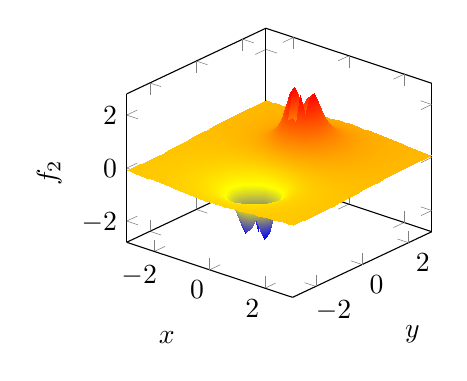
\begin{tikzpicture}
\begin{axis}[width=.45\linewidth,height=5cm,view={40}{30},xlabel={$x$},ylabel={$y$},zlabel={$f_2$},domain=-3:3,y domain=-3:3,samples=35,samples y=35,unbounded coords=jump]
\addplot3[surf,shader=interp] {x^2+(y-1)^2>.09 && x^2+(y+1)^2>.09 ? 1/sqrt(x^2+(y-1)^2)-1/sqrt(x^2+(y+1)^2) : nan};
\end{axis}
\end{tikzpicture}
\end{center}
两图的竖轴是函数值. 奇点周围半径0.3的圆域删去以适应有限图幅, 缺口并非真实平台. 两源模型在$+y$为正峰、$-y$为负峰; 对比第一图的单正峰, 可直观看到奇偶对称和零线.

原第1章场线、位置矢量、圆周运动和余弦定理练习所需的几何关系也可直接建立. 均匀圆周运动$\rr(t)=R(\cos\omega t\,\uv x+\sin\omega t\,\uv y)$给切向速度$\omega R(-\sin\omega t,\cos\omega t)$和向心加速度$-\omega^2\rr$. 对两个矢量$\vct a,\vct b$, $|\vct a-\vct b|^2=a^2+b^2-2ab\cos\theta$来自点积展开. 后面的电荷积分用它计算源到观察点的距离, 并明确其中$\theta$是哪两个矢量的夹角.
